\chapter{Vorbereitung}
Supraleiter zeichnen sich durch eine widerstandslose Leitung unter einer kritischen
Temperatur $T_c$ aus. Die theoretischen Grundlagen hinter 
diesen Effekten sind zahlreich und zum Teil noch Heute ungeklärt. Hier soll ein
kleiner Überblick gegeben werden.

	\section{Theoretische Grundlagen}

    \subsection{Bosonen und Fermionen}
Zum Verständnis der Supraleitung essentiell ist die Unterscheidung der 
Elementarteilchen in Bosonen und Fermionen, sowie die Eigenschaften Dieser.
Für unsere Zwecke genügt es Bosonen und Fermionen zu betrachten.

        \subsubsection{Fermionen}
Als Fermionen werden Teilchen mit halbzahligem Spin ($\frac{1}{2}, \frac{3}{2},
\dots$) bezeichnet. Diese Gruppe der Elementarteilchen, zu der Quarks und 
Leptonen gezählt werden, bildet die Materie.
\vspace{3pt}\\
Für die Supraleitung wichtig ist vor allem das Pauli'sche Ausschlussprinzip, 
welchem Fermionen unterliegen. Es besagt, dass 2 Fermionen am selben Ort nicht
den selben Quantenzustand besetzen dürfen.\\
Dies wird am Beispiel der Elektronen in Atomorbitalen klar. Ohne dieses Prinzip
könnten alle Elektronen im energetisch günstigsten Grundzustand liegen, in Atomen
werden jedoch Besetzungen energetisch höherliegender Zustände beobachtet.
\begin{figure}[h]
    \centering
    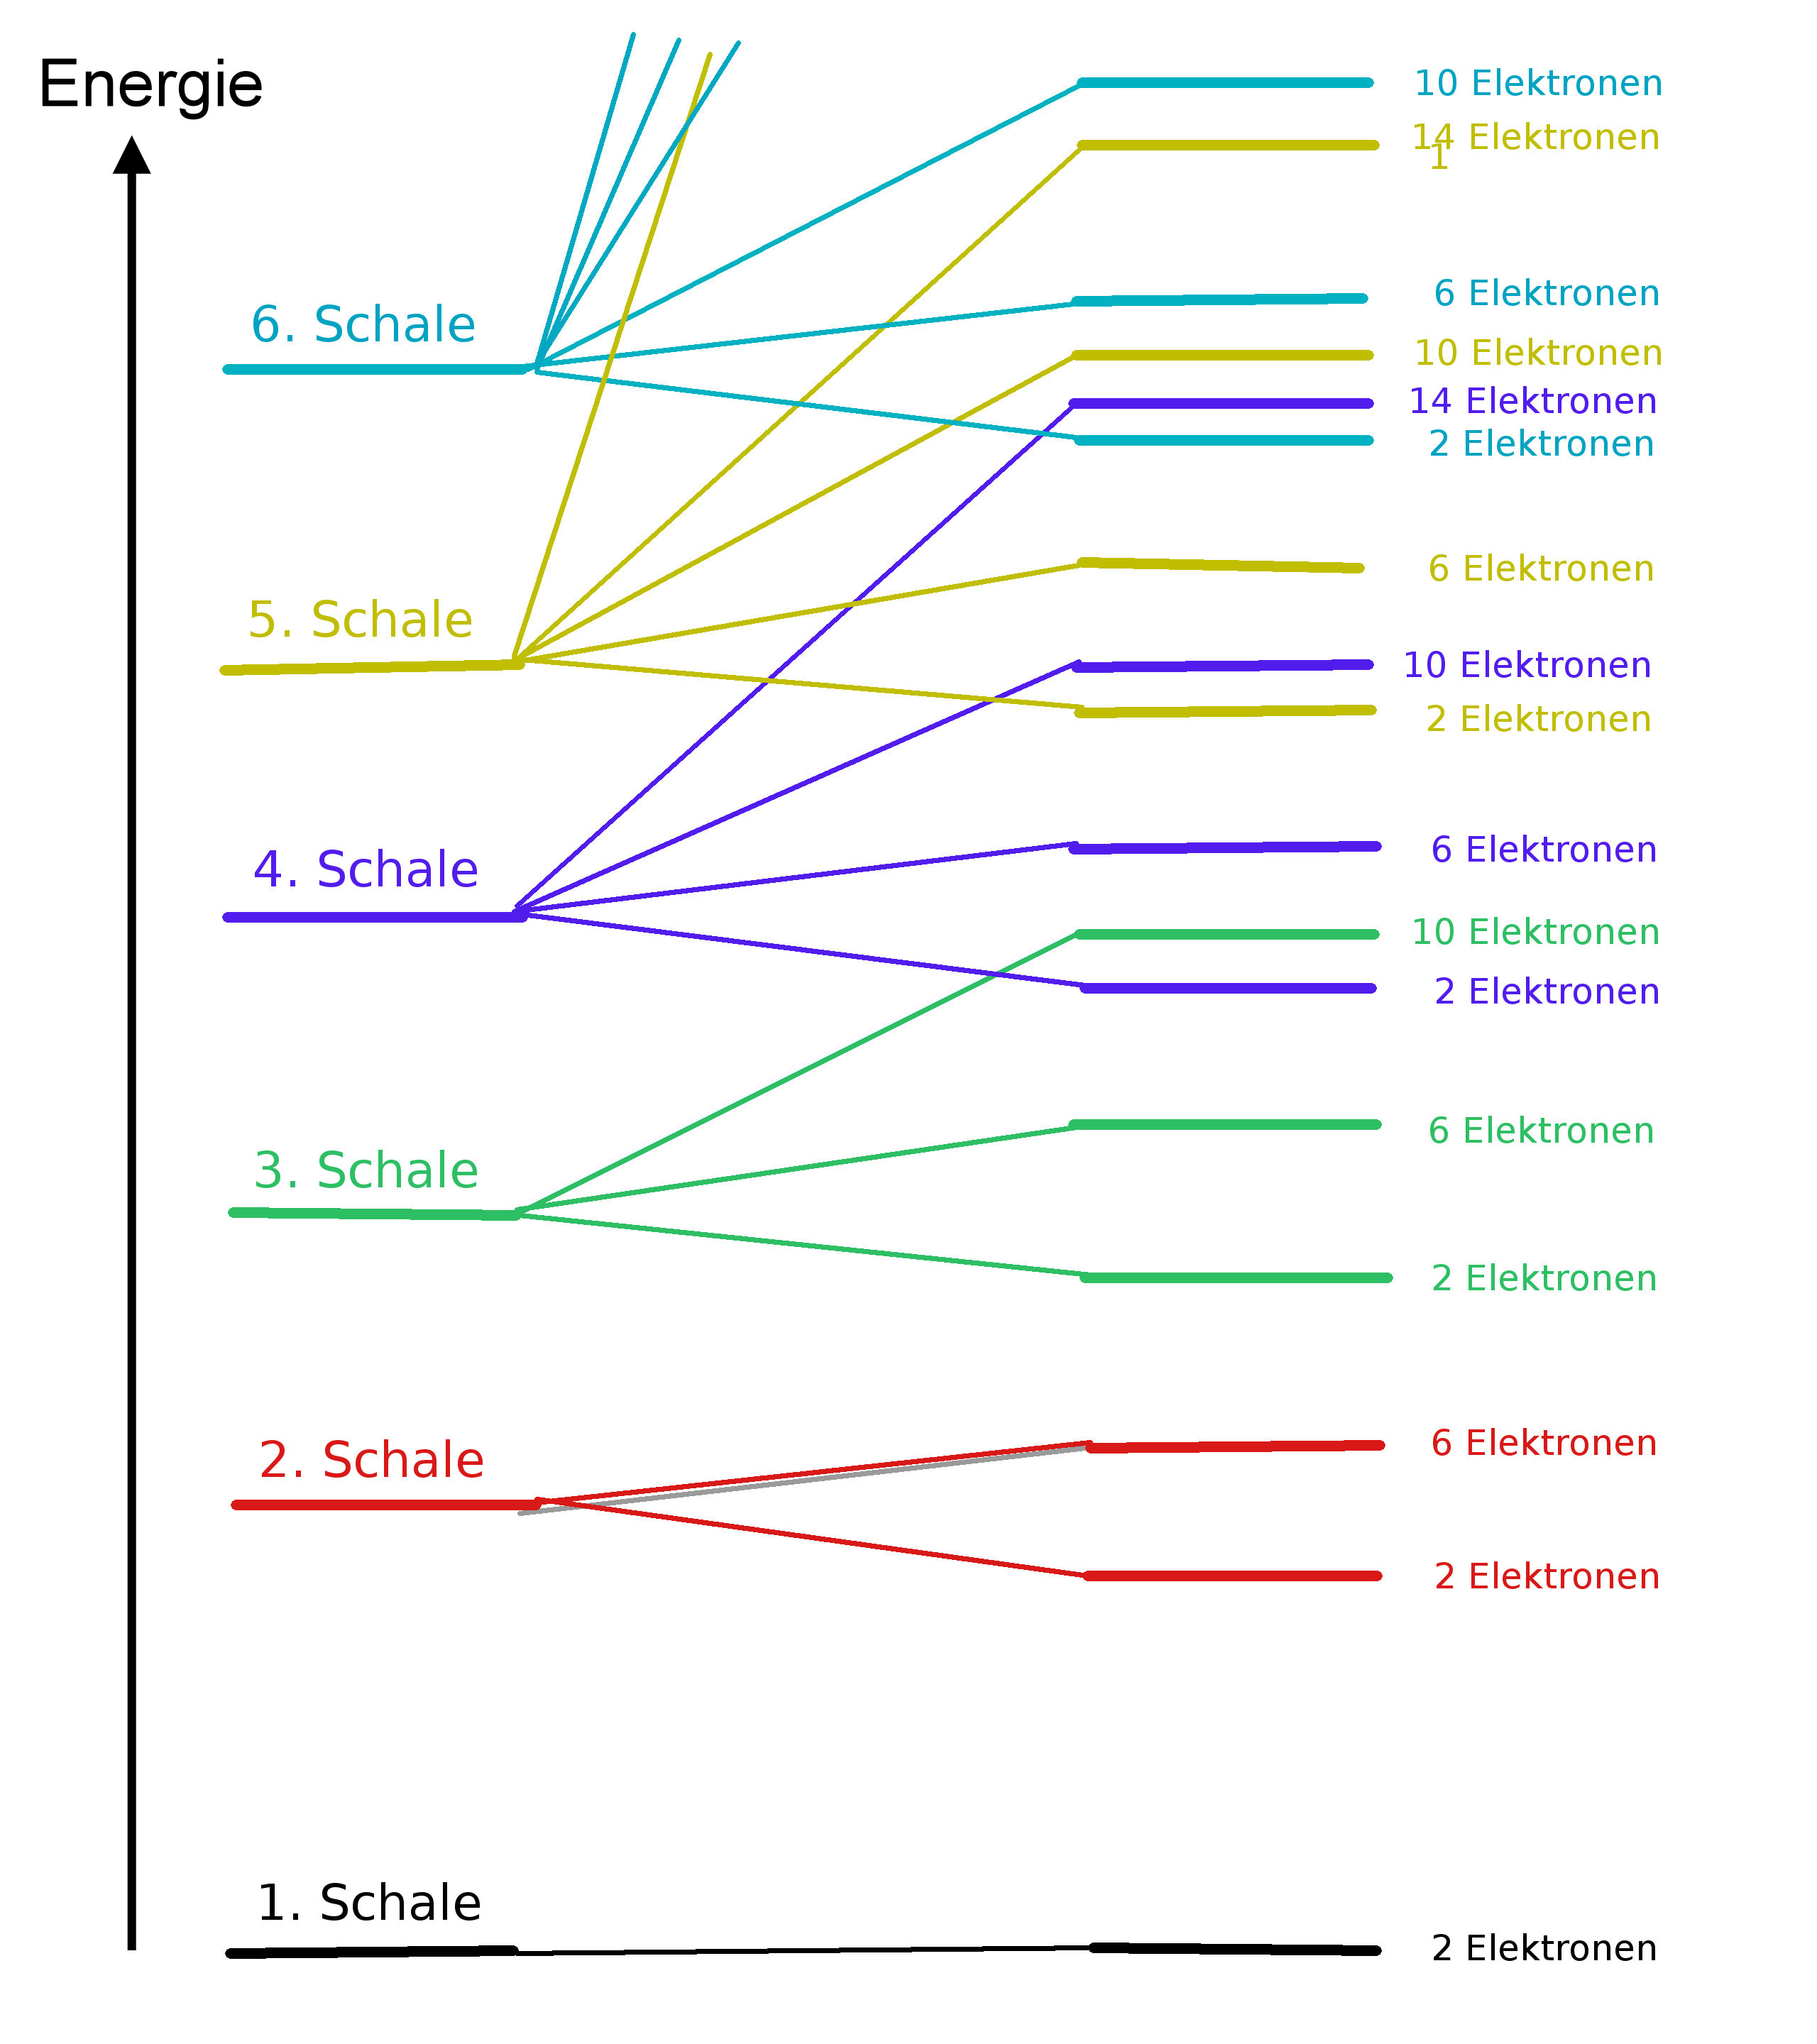
\includegraphics[width=0.4\textwidth]{Abb/energieniveaus-elektronen.jpg}
	\caption{Energieniveaus der Elektronen in Atomorbitalen \cite{energieniveaus}}
    \label{Abb:energieschema}
\end{figure}
In Abbildung \ref{Abb:energieschema} ist die Aufteilung zu sehen. Zuerst werden die
beiden Zustände der ersten Schale besetzt, die sich nur in der Spinausrichtung 
unterscheiden. In den nächsten Schalen werden durch unterschiedliche Drehimpulse 
und Spinausrichtungen der einzelnen Elektronen weitere Zustände besetzt, mit immer
größer werdender Energie. \cite{fermionwiki}

        \subsubsection{Bosonen}
Als Bosonen werden Teilchen mit ganzzahligem Spin bezeichnet. Elementar treten 
Bosonen nur als Austauschteilchen der elementaren Wechselwirkungen zwischen 
Fermionen auf. Ein Beispiel ist hier das Photon als Überträger der 
elektromagnetischen Kraft. Für unsere Zwecke sind jedoch aus Fermionen
zusammengesetzte Bosonen weitaus wichtiger.
\vspace{3pt}\\
Mehrere Fermionen können durch Wechselwirkungen so aneinander koppeln, sodass sie
durch eine gemeinsame Gesamtwellenfunktion beschrieben werden müssen. Einfach
hat dies zur Folge, dass sich Verbunde aus Fermionen, ein bekanntes Beispiel 
hierfür stellen Atomkerne dar, wie Bosonen verhalten. 
\vspace{3pt}\\
Im Gegensatz zu den Fermionen unterliegen Bosonen nicht dem Pauli-Prinzip. Anders
als im obigen Energieschema, ist es also für Bosonen möglich den selben
Energiezustand zu besetzen. Dies wird später für die Theorie der Supraleitung 
essentiell. \cite{bosonwiki}

	\subsection{BCS-Theorie}
Eine gute theoretische Beschreibung Supraleiter 1. Art bietet die BCS-Theorie. 
Zwar kann durch diese die Hochtemperatursupraleitung auch erklärt werden, das 
Prinzip der Paarbildung bleibt jedoch ungeklärt.

        \subsubsection{Cooper-Paare}
Grundlage der Supraleitung ist die Cooper-Paarbildung der Elektronen im Festkörper.
\\
Es wird angenommen, dass ein Elektron, aufgrund seiner negativen Ladung, eine 
Deformationsspur hinterlässt. 
\begin{figure}[h]
    \centering
    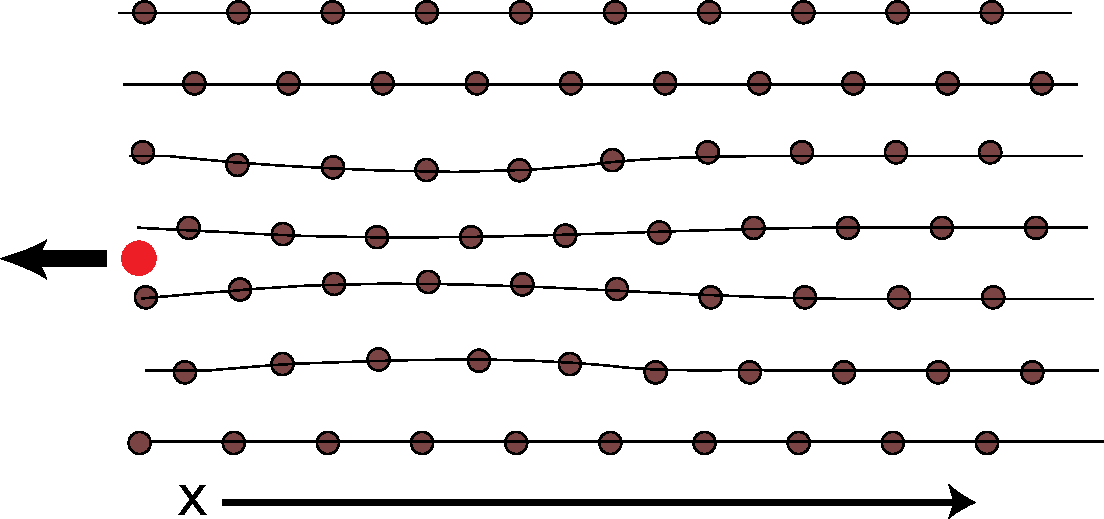
\includegraphics[width=0.7\textwidth]{Abb/deformation.pdf}
    \caption{Deformationsspur hinter einem Elektron \cite{bcswiki}}
    \label{Abb:def}
\end{figure}
Siehe hierzu Abbildung \ref{Abb:def}. Ein Elektron zieht die positiv geladenen Kerne
an, was diese zum Schwingen anregt. Nach einer viertel Schwingperiode erreicht die
Konzentration der positiven Ladungen ihr Maximum und weitere Elektronen werden 
angezogen. Durch die große Reichweite dieser Kraft, das erste Elektron ist nach
einer Viertel Schwingperiode schon weit durch den Festkörper gewandert, wird sie
nicht durch die Coulomb-Abstoßung aufgehoben.
\vspace{3pt}\\
Zur theoretischen Herleitung werden zwei wechselwirkende Elektronen betrachtet, die,
wie oben beschrieben, virtuelle Phononen mit Wellenvektor $\vec{q}$ austauschen.
Die Elektronen mit den ursprünglichen Wellenvektoren $\vec{k}_1, \vec{k}_2$ werden
nun durch $\vec{k}_1' = \vec{k}_1 + \vec{q}$ und $\vec{k}_2 ' = \vec{k}_2 + \vec{q}$
beschrieben. Durch die Impulserhaltung gilt für den Gesamtwellenvektor $\vec{K} =
\vec{k}_1 + \vec{k}_2 = \vec{k}_1' + \vec{k}_2'$.\\
Am absoluten Nullpunkt sind im Festkörper alle Zustände unterhalb von $E_F$
besetzt. Dem Elektronenpaar sind somit lediglich Zustände oberhalb von $E_F$ 
zugänglich. Die attraktive Wechselwirkung spielt sich somit im Energiebereich
$E_F \, - \, E_F + \hbar \omega_D$ ab. $\hbar \omega_D$ ist hierbei die Energie
des Phonons. Betrachtet man diesen Energiebereich im k-Raum beschreibt dieser eine
Kugelschale der Dicke $\delta k = \frac{m \omega_D}{\hbar k_F}$. Anschaulich 
erfüllen für ein vorgegebenes $\vec{K}$ nur Elektronenpaare die Impulserhaltung,
wenn deren Wellenvektor in $\delta k$ anfängt oder endet. 
\begin{figure}[h]
	\centering
	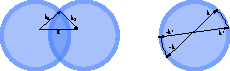
\includegraphics[width=0.8\textwidth]{Abb/cooperstreu.pdf}
	\caption{links: Impulserhaltung der Paarwechselwirkung, rechts: Streuprozess in
			 einem Cooper Paar: der $\vec{K}$ der Schwerpunktsbewegung ist null
			 \cite{hunklinger}}
	\label{streucooper}
\end{figure}
Dies ist in Abbildung \ref{streucooper} dargestellt. Hieraus kann auch gefolgert 
werden, dass der Phononenaustausch für $\vec{K}=0$ am wahrscheinlichsten erfolgt.
Somit gilt $\vec{k}_1 = - \vec{k}_2 = \vec{k}$.\\
Für die Zweiteilchen Wellenfunktion $\Psi (\vec{r}_1,\vec{r}_2)$ bietet sich die 
Verwendung einer Linearkombination von Einteilchenfunktionen zur Lösung an. Da 
$\vec{k}_1 = - \vec{k}_2$, der Schwerpunkt also in Ruhe ist, genügt eine 
Beschreibung durch relative Koordinaten. 
\[
	\Psi ( \vec{r} ) = A \exp ( i \vec{k}_1 \vec{r}_1 ) \cdot \exp( i \vec{k}_2
					   \vec{r}_2) 
					 = A \exp( i \vec{k} ( \vec{r}_1 - \vec{r}_2 ))
					 = A \exp(i \vec{k} \vec{r} )
\]
Durch die ständige Streuung am Gitter in Zustände mit unterschiedlichen 
Wellenvektoren, wird über diese Paarzustände summiert:
\[
	\Psi (\vec{r}) = \sum_{\vec{k}} A_{\vec{k}} e^{i \vec{k} \vec{r}}
\]
$| A_{\vec{k}} |^2$ beschreibt hierbei die Wahrscheinlichkeit ein Elektronenpaar
im Zustand $(k,-k)$ anzutreffen.\\
Bei der Betrachtung des Grenzfalls T=0 gilt für die Wellenzahl der Elektronen 
\[
	\displaystyle k_F < k < \sqrt{\frac{2m(E_F + \hbar \omega_D)}{\hbar^2}}.
\]
$A_k$ verschwindet dann für alle anderen $k$.\\
Weiter muss die Schrödingergleichung mit dem Potential $\tilde{V}(\vec{r}_1,
\vec{r}_2)$, bestehend aus der attraktiven und der abstoßenden 
Coulombwechselwirkung, gelöst werden. Diese langwierige Rechnung wird hier nicht 
weiter ausgeführt. Es wird angenommen, dass das Potential im Energiebereich
$E_F < \frac{\hbar^2 k^2}{2m}, \; \frac{\hbar^2 k'^2}{2m} < E_F + \hbar \omega_D$
den positiven, konstanten Wert $\tilde{V}_0$ annimmt und ansonsten 0 ist. 
Auch wird die Zustandsdichte um die Fermi-Kante als konstant angenommen.\\
Für die Energieänderung im Zuge der attraktiven Wechselwirkung errechnet sich 
\[
	\Delta E = E - 2 E_F = \frac{2\hbar \omega_D}{1- e^{4/(\tilde{V}_0 D(E_F))}}
			 \approx - 2 \hbar \omega_D e^{4/(\tilde{V}_0 D(E_F))}
\]
Im letzten Schritt wurde $\tilde{V}_0 D(E_F) << 1$ angenommen. Die Energie der
Cooper-Paare wird also durch die attraktive Wechselwirkung reduziert.
\\
Grundlage der BCS-Theorie ist nun die Kopplung zweier Elektronen durch diese 
Wechselwirkung, wodurch der Verbund durch eine bosonische Gesamtwellenfunktion
beschrieben werden muss. \cite{bcswiki}, \cite{hunklinger}

		\subsubsection{BCS-Grundzustand}
Als BCS-Grundzustand wird Supraleitung am absoluten Temperaturnullpunkt bezeichnet. 
Zur Konstruktion der Wellenfunktionen werden nun die Paarzustände aus dem 
vorherigen Abschnitt benutzt. Mit der Wahrscheinlichkeit für die Besetzung des
Zustands $(\vec{k} \uparrow, - \vec{k} \downarrow)$ $v_{\vec{k}}^2$, die Spins 
werden hier durch die Pfeile berücksichtigt, kann mit $u_{\vec{k}}^2 = 
1 - v_{\vec{k}}^2$ die Wahrscheinlichkeit, dass ebendieser Paarzustand unbesetzt 
ist, angegeben werden. Zur Gesamtenergie $W_0$ tragen im Grundzustand die kinetische
Energie der Elektronen und die bereits behandelte Wechselwirkungsenergie der 
Paarbildung bei. Somit ergibt sich
\[
	W_0 = 2 \sum_{\vec{k}} v_{\vec{k}}^2 \eta_{\vec{k}} - 
		  \frac{\tilde{V}_0}{V_P} \sum_{\vec{k}, \vec{k}'} v_{\vec{k}} u_{\vec{k'}}
		  						  u_{\vec{k}} v_{\vec{k}'}
\]
Der erste Term beschreibt die kinetische Energie. $\eta_{\vec{k}} = 
\hbar^2 \vec{k}^2/2m - E_F$ gibt hierbei die Abweichung der kinetischen Energie von
der Fermi-Energie an. Die möglichen Spinausrichtungen werden durch den Faktor zwei 
vor der Summe berücksichtigt. Der hintere Term spiegelt die Wechselwirkungsenergie 
wider, die auf der Streuung $( \vec{k} \uparrow, - \vec{k} \downarrow)$ zu 
$(\vec{k}' \uparrow, - \vec{k}' \downarrow)$ beruht.\\
Mit der Abkürzung
\[
	\Delta = \frac{\tilde{V}_0}{V_P} \sum_{\vec{k}'} u_{\vec{k}'} v_{\vec{k}'}
\]
führt die Minimierung von $W_0$ bezüglich $v_{\vec{k}}$ und $u_{\vec{k}}$, unter 
Berücksichtigung des Zusammenhangs $u_{\vec{k}}^2 + v_{\vec{k}}^2 = 1$ zu:
\[
	2 v_{\vec{k}} u_{\vec{k}} \eta_{\vec{k}} - \Delta(v_{\vec{k}}^2 - u_{\vec{k}}^2)
	=0
\]
Mit
\[
	E_{\vec{k}}^2 = \eta_{\vec{k}}^2 + \Delta^2
\]
können die Wahrscheinlichkeitsamplituden zu 
\[
	u_{\vec{k}}^2 = \frac{1}{2} \left( 1 + \frac{ \eta_{\vec{k}} }{E_{\vec{k}}} 
	\right)
	\qquad 
	v_{\vec{k}}^2 = \frac{1}{2} \left( 1 - \frac{ \eta_{\vec{k}} }{E_{\vec{k}}} 
	\right)
\]
umgeformt werden. Für die Energie $W_0$ ergibt sich damit:
\[
	W_0 = \sum_{\vec{k}} \eta_{\vec{k}} \left( 1-\frac{\eta_{\vec{k}}}{E_{\vec{k}}}
		  \right) - \frac{\Delta^2 V_P}{\tilde{V}_0}
\]
Vergleicht man die innere Energie des Normalleiters $W_0^n = 2 \sum_{|\vec{k}| < k_F}
\eta_{\vec{k}}$ mit $W_0$, so ist der Energiegewinn $W_kon = W_0 - W_0^n$, die 
Kondensationsenergie, nach einer Reihe von Umformungen gegeben durch:
\[
	\frac{W_kon}{V_P} = - \frac{1}{4} D (E_F) \Delta^2
\]
Diese Energie wird frei, wenn die Leitungselektronen in den supraleitenden Zustand
kondensieren.

		\subsubsection{Energielücke}
Setzt man in den Ausdruck für die Konstante $\Delta$ aus vorherigem Abschnitt die
Ausdrücke für $u_{\vec{k}}$ und $v_{\vec{k}}$ ein, so erhält man folgenden Term:
\[
	\Delta = \frac{1}{2} \frac{\tilde{V}_0}{V_P} \sum_{\vec{k}} 
			 \frac{\Delta}{\sqrt{\eta_{\vec{k}}^2 + \Delta^2}}
\]
Nach einigen Umformungen und der Annahme, dass die Zustandsdichte um die Fermi-Kante
konstant ist, ist $\Delta$ durch
\[
	\Delta = \frac{\hbar \omega_D}{\sinh \left( \frac{2}{\tilde{V}_0 D(E_F} \right)}
		   \approx 2 \hbar \omega_D e^{-2 / (\tilde{V}_0 D(E_F))}
\]
gegeben. Für den letzte Term wurde angenommen, dass $\tilde{V}_0 D(E_F) << 1$. 
$\Delta$ stellt eine Energielücke im Energiespektrum der Elektronen dar.

		\subsubsection{Widerstandslose Leitung}
Wie bereits erklärt, können die bosonischen Cooper-Paare nun alle den Grundzustand
einnehmen. Dies führt zu einer den ganzen Festkörper überspannenden 
Bose-Einstein-Wellenfunktion, weshalb die Supraleitung als auch makroskopischer
Quantenzustand beschrieben wird. \\
Die widerstandslose Leitung erklärt sich nun durch die Energielücke der Breite 
$E_g$ zwischen dem Grundzustand der Cooper-Paare und dem Gitter. Eine Wechselwirkung
zwischen Elektronengas und Gitter kann nicht stattfinden, solange die 
Elektronenenergie $E_g$ nicht erreicht. Mit dieser Erklärung leuchtet auch die 
Existenz der kritischen Stromstärke $I_c$ und der kritischen Temperatur $T_c$ ein.
Überschreitet die Elektronenenergie durch thermische Anregung, oder auch durch
einen Stromfluss die Energielücke, so brechen die Cooper-Paare auf und der 
Festkörper geht wieder in den normalleitenden Zustand über. \cite{hunklinger}, 
\cite{suprawiki}

	\subsection{Meisner-Ochsenfeld Effekt}
Eine weitere wichtige Eigenschaft eines Supraleiters ist sein Verhalten im 
Magnetfeld. Dieses wird durch den Meisner-Ochsenfeld Effekt beschrieben.
\begin{figure}[h]
	\centering
	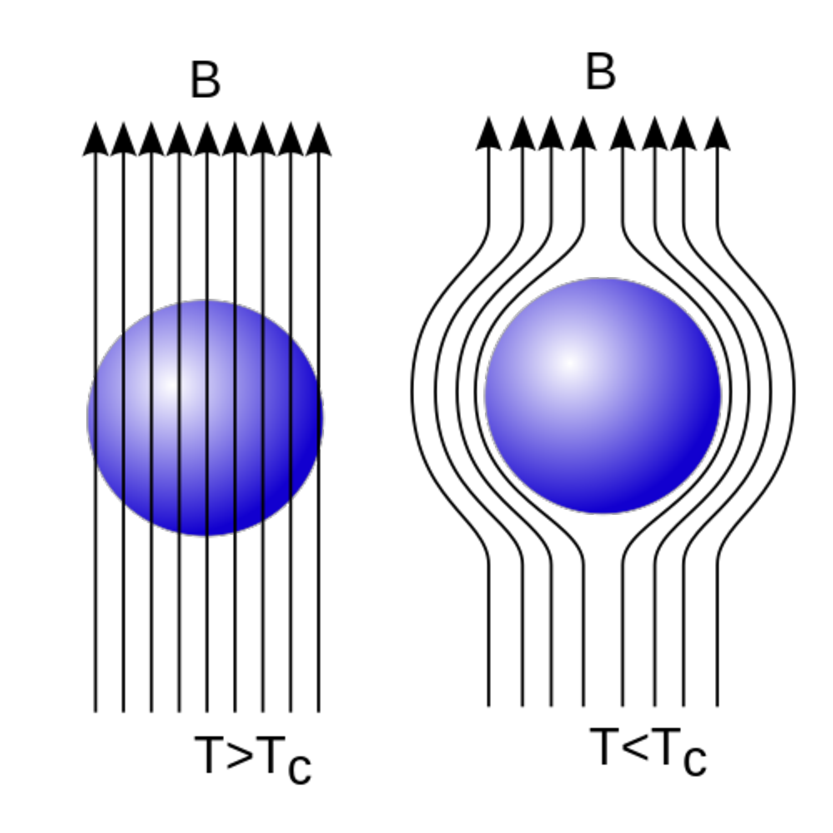
\includegraphics[width=0.6\textwidth]{Abb/meisner.pdf}
	\caption{Magnetfeld um einen Supraleiter vor und nach Abkühlung unter $T_c$ 
	\cite{meisnerwiki}}
	\label{Abb:meisner}
\end{figure}
Wie in Abbildung \ref{Abb:meisner} zu sehen, wird ein Magnetfeld, das oberhalb der
kritischen Temperatur $T_c$ den Festkörper durchdringt, in der supraleitenden Phase
aus dem Leiter verdrängt wird. Hier wird in einer dünnen Schicht unter der 
Oberfläche ein Abschirmstrom induziert, der die Feldlinien des äußeren Feldes aus
dem Material verdrängt. Der Supraleiter ist also ein idealer Diamagnet. Dieser 
Effekt wird als Meisner-Ochsenfeld Effekt bezeichnet. \cite{hunklinger}, 
\cite{meisnerwiki}

		\subsubsection{Typ-I Supraleiter}
Diese Art funktioniert genau wie in Abbildung \ref{Abb:meisner} gezeigt. In der 
supraleitenden Phase wird das Feld aus dem Inneren verdrängt. Die Normalleitung 
wird durch eine Temperatur größer $T_c$, einen Strom größer $I_c$, oder ein
Magnetfeld stärker als die kritische Feldstärke $B_c$ wiederhergestellt. 
\cite{hunklinger}

		\subsubsection{Typ-II Supraleiter}
Bei diesen Materialien gibt es eine untere kritische Feldstärke $B_{c1}$. Oberhalb
dieser dringt das Magnetfeld in Form von Flusschläuchen, wie in Abbildung 
\ref{Abb:flusschlauch} zu sehen, in den Festkörper ein. Der elektrische Widerstand
bleibt jedoch weiterhin sehr klein.
\begin{figure}[h!]
	\centering
	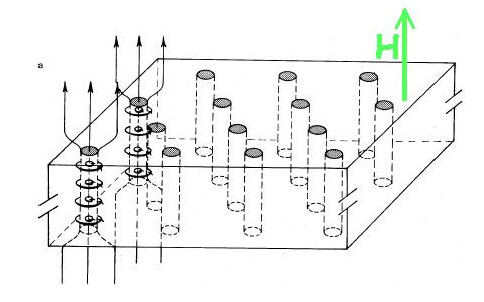
\includegraphics[width=0.6\textwidth]{Abb/flussschlauch.jpg}
	\caption{Flussschläuche im Typ-II Supraleiter oberhalb von $B_{c1}$ 
		     \cite{flussschlauchbild}}
	\label{Abb:flusschlauch}
\end{figure}
Übersteigt die Feldstärke den Wert der kritischen Feldstärke $B_{c2}$, so geht
der Supraleiter endgültig in die normalleitende Phase über. \cite{hunklinger}

	\section{Messtechnische Grundlagen}

		\subsection{Vier-Punkt-Methode}
\begin{figure}[h]
	\centering
	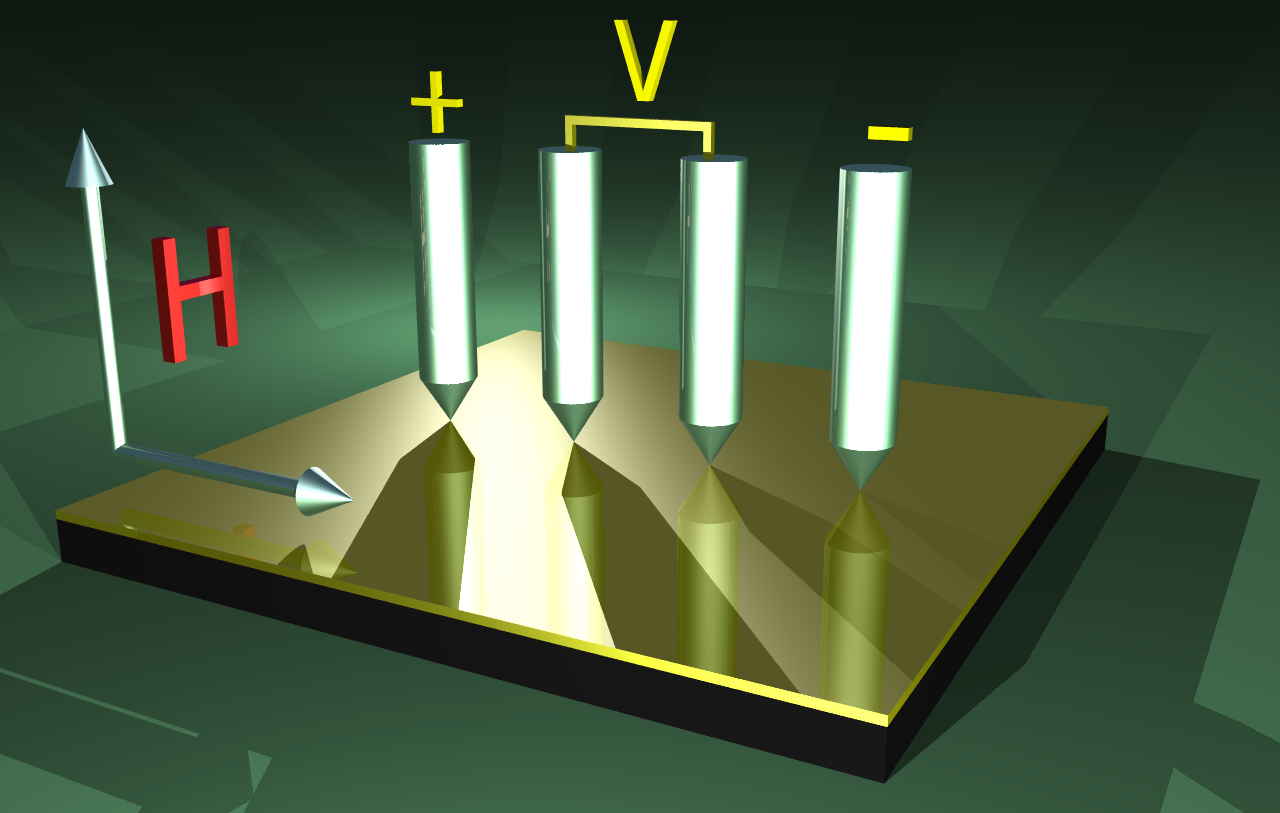
\includegraphics[width=0.6\textwidth]{Abb/vierpunkt.png}
	\caption{Vier-Punkt-Methode \cite{vierpunktwiki}}
	% Von Maciej UMacieju - Eigenes Werk, Gemeinfrei, https://commons.wikimedia.org/w/index.php?curid=2114288
	\label{Abb:vierpunkt}
\end{figure}
Zur Minimierung von Störwiderständen bei der Messung, wird die Vier-Punkt-Methode 
verwendet. Hierbei wird die Probenoberfläche mit vier Messspitzen kontaktiert. An
den beiden äußeren Kontakten wird ein Strom angelegt, während an den Inneren eine
Spannung gemessen wird. Der Aufbau ist in Abbildung \ref{Abb:vierpunkt} zu sehen.
Durch den sehr großen Innenwiderstand des Spannungsmessers kann der Widerstand
durch das Ohm'sche Gesetz berechnet werden. \cite{vierpunktwiki}, 
\cite{vierleiterwiki}

		\subsection{Thermoelement}
Zur Temperaturmessung wird ein Paar aus verschiedenen metallischen Leitern am Ende
verbunden. Durch den thermoelektrischen Effekt treten bei einer Temperaturänderung
im Inneren der Metalle Ströme auf.
\begin{figure}[h]
	\centering
	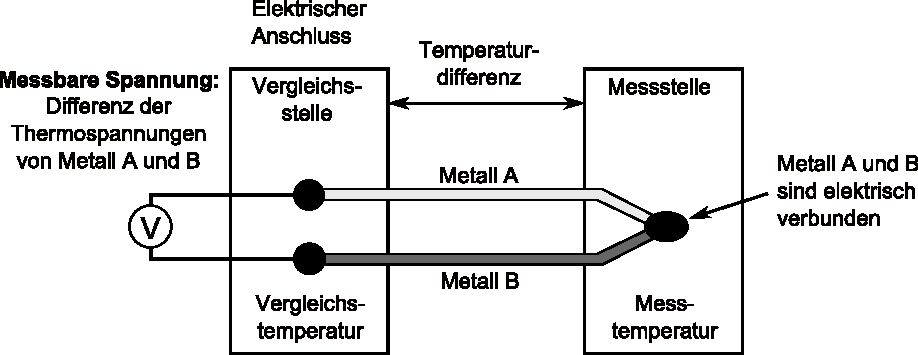
\includegraphics[width=0.8\textwidth]{Abb/thermo.pdf}
	\caption{Aufbau eines Thermoelements \cite{thermowiki}}
	\label{Abb:thermo}
\end{figure}
Man misst nun, wie in Abbildung \ref{Abb:thermo} dargestellt die Differenz der 
Thermospannungen in den beiden Metallen. Mithilfe der Referenztemperatur kann nun
hieraus die Temperatur an der Messstelle berechnet werden. \cite{thermowiki}

		\subsection{Lock-In Verstärker}
Der Lock-In Verstärker wird zur Signalverstärkung und Säuberung, gerade bei 
schwachen Messsignalen, eingesetzt. Effektiv wirkt er wie ein extrem schmalbandiger
Bandpassfilter.
\begin{figure}[h]
	\centering
	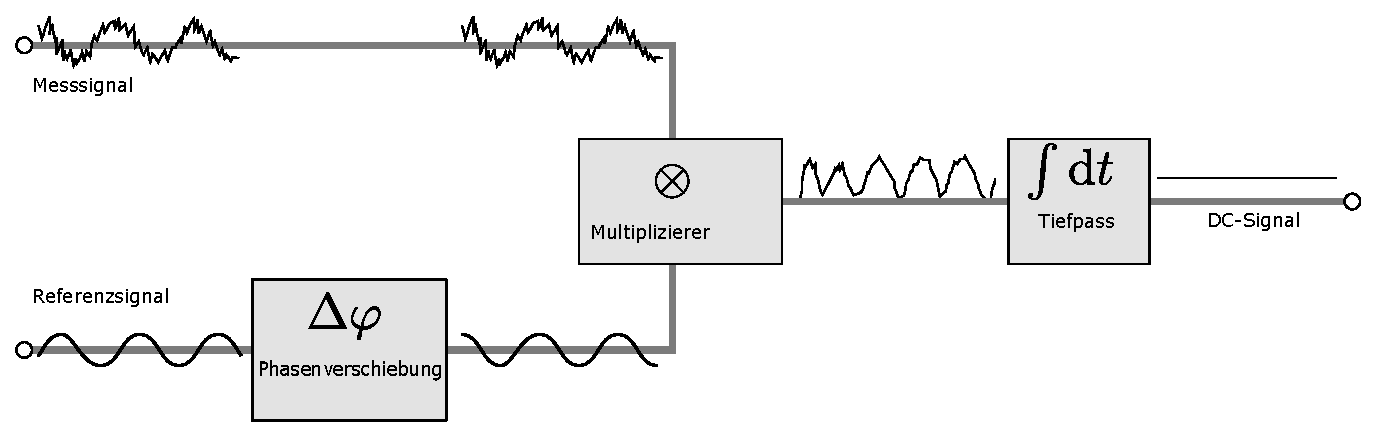
\includegraphics[width=0.7\textwidth]{Abb/lockin.pdf}
	\caption{Schematischer Aufbau eines Lock-In Verstärkers \cite{lockinwiki}}
	\label{Abb:lockin}
\end{figure}
Der schematische Aufbau ist in Abbildung \ref{Abb:lockin} zu sehen. Das Messsignal
wird mit einem Referenzsignal multipliziert, dessen Phase zuvor verschoben werden 
kann. Anschließend wird durch einen Tiefpass integriert. Unterscheiden sich die 
Frequenzen der Messung und der Referenz, so liefert die Integration null. Durch
Variation der Referenzfrequenz kann also ein bestimmter Anteil des Messsignals
"gelockt" werden. \cite{lockinwiki}, \cite{kreuzwiki}
